\documentclass[crop,tikz,12pt]{standalone}

\usepackage{tikz-qtree}
\usetikzlibrary{arrows.meta}
\usetikzlibrary{decorations.text}

\definecolor{bg1}{RGB}{244,231,195}
\definecolor{bg2}{RGB}{234,204,161}
\definecolor{l1}{RGB}{209,148,106}


\begin{document}

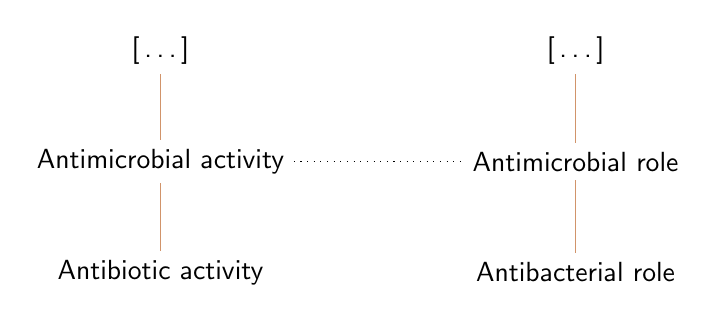
\begin{tikzpicture}[
    level distance=4em,
    sibling distance=2em,
    every tree node/.style={
        align=center, font=\sffamily
    },
    edge from parent/.append style={
        line width=0,
        color=l1
    },
    edge from parent path={
        (\tikzparentnode.south) -- +(0,-1em) -| (\tikzchildnode)
    },
    every edge/.append style={
        dashed, draw=l1,
        -{Computer Modern Rightarrow[] . Computer Modern Rightarrow[]}
    },
    b/.append style={
        {Computer Modern Rightarrow[] . Computer Modern Rightarrow[]}%
        -{Computer Modern Rightarrow[] . Computer Modern Rightarrow[]}
    },
    l/.style={
        fill=white,inner sep=0.7mm,node font=\scriptsize\itshape
    }
]

    \Tree   [ .{[\kern \fontdimen 3\font\ldots]}
                [ .\node(one){Antimicrobial activity};
                    {Antibiotic activity} ] ];
    \begin{scope}[shift={(15em,0pt)}]
    \Tree   [ .{[\kern \fontdimen 3\font\ldots]}
                [ .\node(two){Antimicrobial role};
                    {Antibacterial role} ] ];
    \end{scope}
    \draw[dotted] (one) -- (two);
    
\end{tikzpicture}

\end{document}





